\section{Literature Review}
\subsection{Theoretical Background}
In order to fully grasp the impact of controversy in the LM training and its performance, it is really essential to first get a clear view and understanding of the theoretical concepts behind the following areas:(Language Model Training, Bias in Language Models, Controversial Source Data)

Language models by themselves are an essential part of Natural Language Processing. These models work by the following logic: estimating the likelihood of the words based on the ones that came before it, which gives them the opportunity to produce text that is kinda similar to natural human language. After, they are getting exposed to huge quantities of income data for the reason, that it can train these models by acquiring knowledge of the patterns and connections between words and sentences and even the whole logic in the text, depending on chosen techniques and strategies. 

Bias exhibition in a model means, the demonstration of a tendency to favor particular outputs influenced by patterns that are determined during the training phase. In case, training data incorporates systematic prejudices or favoritism tied to gender, race, age, or other distinguishing features for classifying people into groups, the model could be inadvertently absorbing and propagating exactly these biases.\cite{TB2016}



Controversial Source Data refers to a wide variety of text-based information that’s like a Pandora's box of discussion and debate. Such kind of data includes mostly content characterized by its sensitivity, challenge, and even the shock content. The overall variety of controversial source data, will be inverstigated in this research, due to the reason, that a lot of different studies classify the types in different ways because there is stil, no exact definition of it due to controversy in itself.\cite{dh2016} But it's also shoud be crucial to remember that 'controversial' doesn't always mean ‘bad’ or ‘useless’’. Such kinds of sources are tagged as  controversial because they in reality they cause passionate debates and plenty of different views. They could be sensitive or even potentially offensive in some cases, or just tap a little into a topic that society often disagrees with.

At the heart of AI ethics, there are a lot of significant questions are raised : shouldt we truly educate language models by adding this disputable data? In that case, how does it affect on LM functionionality and more important, what are the ethical consequences of that? The main focus is on exploration how the reliance and performance of language models are influenced by controversial source data.


Understanding the foundational concepts above is the first step in investigation how controversial source data can impact language model performance and possible strategies to mitigate thiese drawbacks. In the following sections we will delve into each topic, examining the existing researches and checking which areas require further exploration.  

\subsection{Training Language Models} 
In order to easily comprehend everything what is written about in this research, it is crucial to understand the training process of language models in general, and also what is “normal” data and what is the difference between these “types”. During training, LM absorbs huge amount of data and learns how to predict the specific output via extracting the features of dataset. The most important part of training is the process of 'backpropagation', which involves iteratively updating model’s parameters in order to minimize the difference between its predictions and the real values.   \cite{KGK2016}

As it was discussed before there is such type of training data that considered as controversial, but now it is time to shift attention to 'standard' source data type, that comes from an extensive collection of texts that truly captures the whole range found in a human language usage. It covers a wide range of different topics and viewpoints without showing subjective preference towards any specific point of view or subject. Moreover, investigations into such kind of data have discovered a blend of digital texts, that now considered as approved or verified sorces, spanning from books and school articles to big websites and social media posts.   \cite{jd2019}

However, it shouldnt be considered that if the data tagged as normal there is no bias or perspectives, while it may seems to everybody that LM represents language usage in the real world, it can hide societal biases or contentious elements. Which leads us to more specified topic: the impact of controversial aspects within 'standard' data on the training and effectiveness of language models. \cite{TB2016}

\subsection{Controversial Source Data: Definition and effect}
Now it is time to reveal all types of data that can be considered controversial, as it was noticed before, controversial source data is not just a data type that has controversy of viewpoints inside of it or the reason of causing of so many debates in society. Controversial source data can be met in the following cases:
\subsubsection{Hate speech and offensive language}Hate speech and offensive language refer to the category of language that includes words or whole phrases that express extreme dislike or violence against some people or groups based on elements that distinguish them from each other such as their race, religion, ethnicity, or even gender. It can range from small slurs and derogatory expressions to real harsh curse words that can make even an adult cry.
Unfortunately, there is an issue surrounding the inclusion of such kinda content during the training phase. Of course, despite the fact that it takes into account the diversity of language usage, at the same time it carries a high risk of obtaining results reflecting offensive or harmful statements. Consequently, without sufficient supervision applied to the selection and management of training data sets, these models may not in purpose reinforce social biases and stereotypes that exist within marginalized communities. Essentially speaking, if the hate speech would be allowed to stay within their training data sets unchecked, most probably the language model will gain and propagate patterns and features causing hateful speech, thus further sharing and spreading its negative effects in our society.\cite{tdd2017}
\subsubsection{News Articles and Political Propaganda}
Propaganda, often spread through speeches, news articles, and social media posts, aims to influence public opinions and beliefs, usually to promote a specific political agenda. It can be biased, misleading, or even false, potentially sowing discord or distrust. If used as training data, it can teach language models to parrot similar divisive or biased viewpoints, thus undermining democratic processes and the free exchange of ideas.

The main aim of these methods of information dissemination is to change the opinion of society in their favor, as well as to encourage people to do certain actions beneficial to the one who spread everything initially, in a political sense, propaganda has always meant to control public opinion in order to convince people of something certain. These data types are considered to be cotroversial since in most cases they include bias and often they spread misleading or even false information in purpose. 

As example lets take a situation where you or somebody else is reading a book that only tells the story from only one perspective. In case if it is the only book you read, it is really possible that you might end up believing that one-sided perspective that was gained from  book is the complete truth because there is nothing to compare with. Let's say that this one-sided book was chosen as a representative of some book genre and thus will be used as training data. Then, the model that learned on it , just like the person reading the book, will learn only from exactly that one perspective. It would then generate outputs that echo this bias, which can contribute to further spreading of skewed perspectives or misinformation.

A real-world example of this is seen in the study by Allcott and Gentzkow (2017)\cite{ha2017}. The researchers dedicated their efforts to comprehensively exploring how social media impacted the proliferation of fake news throughout the course of the 2016 U.S election. Their investigation has done significant findings – false news articles in favor of Donald Trump were widely shared with an astonising count totaling 30 million instances. Far surpassing Hillary Clinton favorably inclined stories that were shared merely eight million times more. This study primarily sought to shed light on social medias role in facilitating the spread of misleading or fabricated narratives; however.  It brought the forth an important realization - politically biased information has considerable power over shaping public opinion. Should we rely on such imbalanced data to train language models we inadvertently risk perpetuating and amplifying these biases and distortions.
\subsubsection{Texts from Historical or Religious Documents}

These sources mostly include literature from significant cultural, historical, or art works, which provide valuable info about our past and cultural development, but in today's realities it can be considered controversial because of the works that could present stereotypes or points of view that are no longer accepted by society because of shifting social norms and standards through time. Without proper context or care, including them in training data could lead to models producing offensive or insensitive outputs, which might be ok in past times, but in the modern world no more concerned. For instance, in ancient times women with blond hair were considered as witches, thus burned, but if we look at the situation today, no one expresses a desire to kill a person with a different hair colour, as for many people it may even seem absurd.


\subsubsection{User-Generated Content from Forums or Online Communities}

Online and Social media mostly consist of all user-generated content, where a huge range of topics are discussed from different viewpoints. Not always, but the chance that this data can be controversial is really big, due to inherent biases, potential misinformation, or even hate speech present. If such content is incorporated into the training data. It has the potential to introduce comparable biases and inaccuracies into the language model that is being trained. This could perpetuate harmful stereotypes or spread misinformation.

For instance in February 2023, the so-called developer Noble Ackerson wanted to check the GPS for its reliability and decided to ask him casual questions to identify weaknesses\cite{na2023}. As it was easy to guess, the language model could not answer all the questions correctly, with such a review, the researcher began to ask questions about himself, since he could confirm this information in any case. The most interesting thing happened when Noble requested information about himself, and got response as Noble Ackerson died in 2019, which is unreal because the article couldn't posted itself. As an explanation , it is possible that information from different sources that ever existed about him got probably mixed with a person who has the same name. This example, shows that some information in ChatGPT is not reliable, therefore it proves an existence of controversial data points in training dataset. Even in case when some people think that this mistake happened just because of non popularity topic or character of the request, then on another example, Noble demonstrated a new request related to Olympic games, where LM again made a mistake with a year when this event occured. 

\begin{figure}
\centering
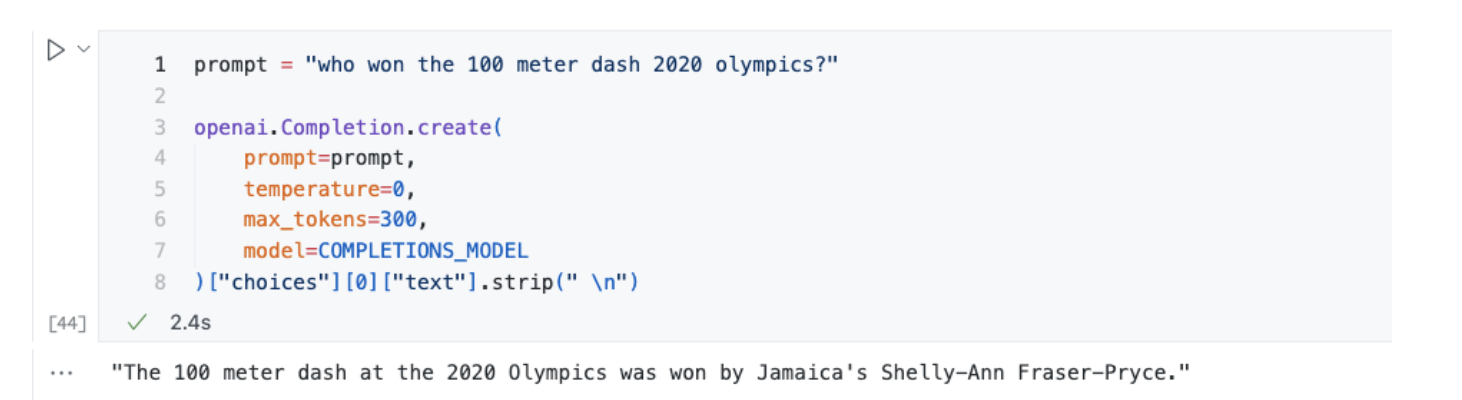
\includegraphics[width=1\textwidth]{Seminararbeit_KI-BA/pic2.png}
\caption{\label{fig:frog}An example to highlight factual accuracy (i.e., hallucinations or confabulation). Prompt: “who won the 100-meter dash 2020 Olympics?”}
\end{figure}